\documentclass[10pt,twocolumn]{article}
\usepackage{graphicx}
\usepackage[margin=0.5in]{geometry}
\usepackage[cmex10]{amsmath}
\usepackage{array}
\usepackage{booktabs}
\usepackage{mathtools}
\title{\textbf{Optimization Assignment - 1}}
\author{A L U R U A J A Y}
\date{September 2022}


\providecommand{\norm}[1]{\left\lVert#1\right\rVert}
\providecommand{\abs}[1]{\left\vert#1\right\vert}
\let\vec\mathbf
\newcommand{\myvec}[1]{\ensuremath{\begin{pmatrix}#1\end{pmatrix}}}
\newcommand{\mydet}[1]{\ensuremath{\begin{vmatrix}#1\end{vmatrix}}}
\providecommand{\brak}[1]{\ensuremath{\left(#1\right)}}
\providecommand{\lbrak}[1]{\ensuremath{\left(#1\right.}}
\providecommand{\rbrak}[1]{\ensuremath{\left.#1\right)}}
\providecommand{\sbrak}[1]{\ensuremath{{}\left[#1\right]}}

\begin{document}

\maketitle
\paragraph{\textit{Problem Statement} - An aeroplane can carry a maximum of 200 passengers.A profit of Rs.1000 is made on each executive class ticket and a profit of Rs.600 is made on each economy class ticket. The airline reserves at least 20 seats for executive class. However, at least 4 times as many passengers prefer to travel by economy class than by the executive class. Determine how many tickets of each type must be sold in order to maximise the profit for the airline. What is the maximum profit?} 
\section{Solution}
Let Number of Executive class ticket sold be x
\vspace{0.3cm}\\
Let Number of Economy class ticket sold be y
\vspace{0.3cm}\\
According to Question
\vspace{0.3cm}\\
Aeroplane can carry maximum 200 passengers
\begin{align}
    x+y \leq 200
    \vspace{0.3cm}\\
    \myvec{1\\1}\vec{x}\leq 200
\end{align}
Since, atleast 20 tickets is reserves for executive class
\begin{align}
  x \ge 20  
  \vspace{0.3cm}\\
\myvec{1\\0}\vec{x}\ge 20
\end{align}
Since the number of tickets for economy class should be at least 4 times the executive class
\begin{align}
    y - 4x \ge 0
    \vspace{0.3cm}\\
     \myvec{-4\\1}\vec{x}\ge 0
\end{align}
Also, the number of tickets can't be negative,so
\begin{align}
    x \ge 0 \And y\ge 0
    \vspace{0.3cm}\\
    \myvec{1 \\ 0} \vec{x} \ge 0
      \vspace{0.4cm}\\
    \myvec{0 \\ 1} \vec{y} \ge 0
\end{align}
\begin{flushleft}
The above equations in vector form is :
\begin{align}
\vec{A_1} = 
\begin{pmatrix}
1 \\
1 \\
\end{pmatrix} \\
\vec{A_2} = 
\begin{pmatrix}
1 \\
0 \\
\end{pmatrix} \\
\vec{A_3} = 
\begin{pmatrix}
-4 \\
1 \\
\end{pmatrix} \\
\vec{A_4} = 
\begin{pmatrix}
1 \\
0 \\
\end{pmatrix} \\
\vec{A_5} = 
\begin{pmatrix}
0 \\
1 \\
\end{pmatrix} \\
\end{align}
\begin{flushleft}
which can be expressed in vector form as
\end{flushleft}
\begin{align}
 \myvec{-1 &-1 \\ 1 & 0 \\ -4 & 1 \\} \vec{x}\ge \myvec{200 \\ 20 \\ 0}
\end{align}
Let P be the maximum number of tickets of each type must be sold in order to maximise the profit for the airline . The problem can be formulated as
\end{flushleft}
\begin{align}
	P = \max_{x,y}(x+y)
\end{align}
The optimization is done by using cvxpy packges in python language:
\begin{align}
	P_{max} = 136000 \\
	\vec{x} = \myvec{40 \\ 160}
\end{align}

\section{Graph}

\begin{figure}[h]
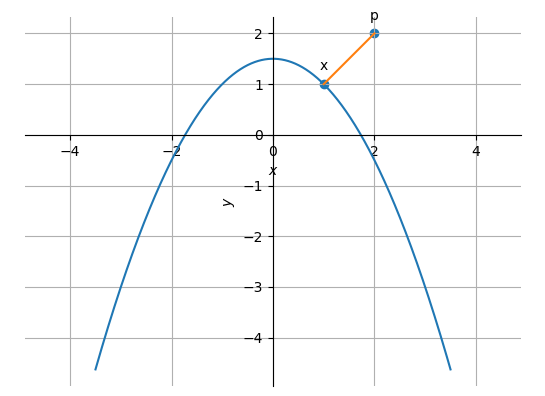
\includegraphics[scale=0.3]{opt.png}
\caption{Graph}
\label{fig:Graph}
\end{figure}

\end{document}






